\section{WebKit}
\label{sec:webkit}

\par \emph{WebKit} is a layout engine software designed to allow web browsers to render html (is not only on web pages). Become a FLOSS project in 2005 when Apple released the code.

\par Is used in Mac OS X system framework with Safari, Dashboard, Mail, and many other OS X applications. Also you can find WebKit in Nintendo 3Ds, Kindle and Android.

\par This project started as a branch of the KHTML and KJS libraries from KDE. It is a community made ​​up by companies: Apple, Nokia, Google, RIM, Igalia, Samsung. Because most contributions are made by companies, I want to emphasize that the company that provides more code to WebKit is Google.It is strange to see this information on a project controlled by Apple.

\begin{figure}[H]
    \centering
    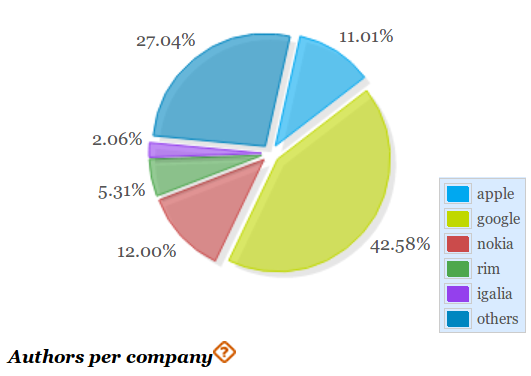
\includegraphics[width=0.7\textwidth]{bitergia-webkit}
    \caption{Bitergia WebKit analysis: \url{http://bitergia.com/public/reports/webkit/2013_01/}}
    \label{}
\end{figure}

\par You can see better numbers in the study by Bitergia on WebKit community posted on February 6, 2013,\textbf{ \href{http://blog.bitergia.com/2013/02/06/report-on-the-activity-of-companies-in-the-webkit-project/}{Bitergia blog}}.

\subsection{Technologies}

\par Documentation :The technologies surrounding the WebKit project, which we consider as ALM Tools, (Application Lifecycle Management):

\begin{itemize}
	\item Bug Tracking System (BTS) Bugzilla - \url{https://bugs.webkit.org/}
	\item Issue Tracking System (ITS) Trac - \url{http://trac.webkit.org/}
	\item Early Warning Systems (EWS) Bugzilla - \url{http://webkit-commit-queue.appspot.com/}
	\item Developer Guides for each Operative System - \url{http://www.webkit.org/building/tools.html}
\end{itemize}

\par I will highlight as the \textbf{EWS} tool. \textit{EWS} offers a tracking code contribution we have made to the project (via a patch). It reflects the results of each test in each type of platform. WebKit looks much the appearance of the test because a change can affect millions of users.

\par As we can see, the system shows a first image of the \textbf {\href{http://webkit-commit-queue.appspot.com/}{status of contributions}}.

\begin{figure}[htp]
    \centering
    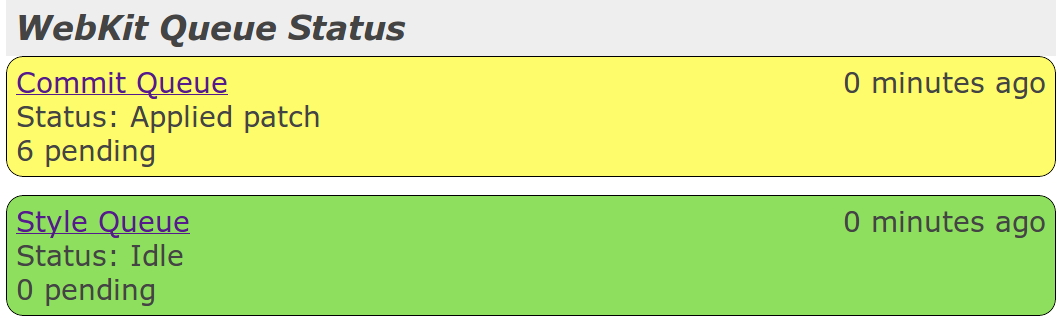
\includegraphics[width=0.7\textwidth]{webkit-queue-status}
    \caption{Queue status}
    \label{queue-status}
\end{figure}

\par Accessing   \textbf {\href{http://build.webkit.org/console}{BuildBot WebKit Console}}, we have access to the results and follow-up of each of the patches and tests for each of the existing distributions (ports).

\begin{figure}[htp]
    \centering
    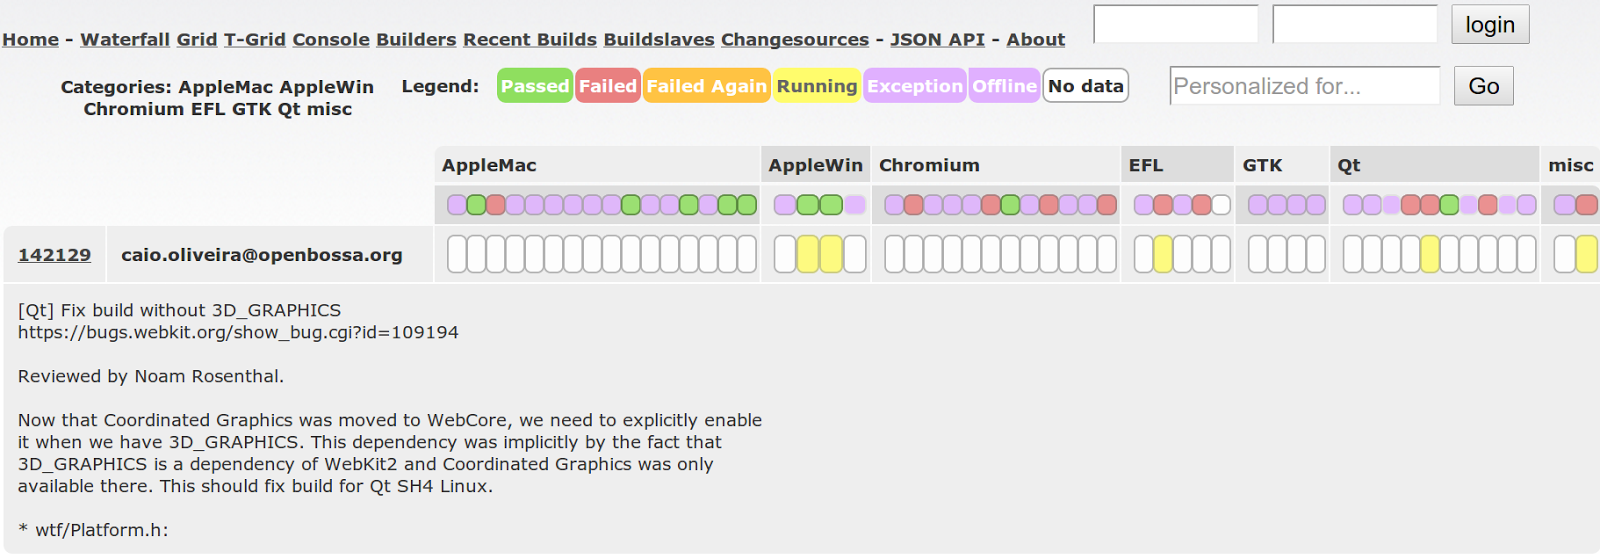
\includegraphics[width=0.7\textwidth]{webkit-build-bot.png}
    \caption{Webkit build bot}
    \label{build-bot}
\end{figure}

\par It is very rigorous system of contributions to the project, we will see in the next section.

\par WebKit has a very useful development guidelines documentation:

\begin{itemize}
	\item \textit{Coding style guidelines} - \url{http://www.webkit.org/coding/coding-style.html}
	\item \textit{Technical Articles} - \url{http://www.webkit.org/coding/technical-articles.html}
	\item \textit{Regression Testing} - \url{http://www.webkit.org/quality/testing.html}
	\item \textit{Reporting Bugs} - \url{http://www.webkit.org/quality/reporting.html}
	\item \textit{Bug Life Cycle} - \url{http://www.webkit.org/quality/lifecycle.html}
	\item \textit{Wiki Documentation} - \url{http://trac.webkit.org/wiki}
\end{itemize}

\subsection{How to Contribute}

\par In WebKit there are many ways of contributions; translations, code, documentation, etc. We are going to focus on contribute with code.
\par There is a guideline explaining  \textbf {\href{http://www.webkit.org/coding/contributing.html}{how to contribute code}}. These are the steps you have to follow to contribute code in WebKit:
\begin{itemize}
	\item Choose or create a bug report to work on.
	\item Develop your changes.
	\item Make sure your changes meet the code style guidelines. The check-webkit-style script may be of help.
	\item Run the layout tests using the run-webkit-tests script and make sure they all pass. See the testing page for more information, as well as what you need to do if you've modified JavaScriptCore.
	\item Add any new files to your working directory.
	\item Prepare a change log entry. You may have to add entries to multiple ChangeLogs. The prepare-ChangeLog script will create stub entries for you. See the paragraph about ChangeLogs below.
	\item Create the patch using the svn-create-patch script.
	\item Submit your patch for review to bugs.webkit.org.
	\item Make any changes recommended by the reviewer.
	\item Once reviewed, ask someone to land your patch or mark it for automated commit.
	\item Please watch for any regressions it may have caused (hopefully none)!
\end{itemize}

\subsubsection{Committers and Reviewers}

\par WebKit contributors are divided into two groups; \textit{committers} and \textit{reviewers}. The committers can contribute code to the reviewers agree.

\par \textit{To be a committer}, you have to be nominated by the reviewers. Having a minimum number of significant patches \textit{(ranges between 10 and 20)}. Bureaucratic process and receive approval of 3. Is searching the plurality of contacting between one or more reviewers.

\begin{quotation}
    \textit{Any company with more than three reviewers may give permission to a reviewer.}
\end{quotation}

\par Becoming reviewer, is a higher jump. You have been elected by \textit{reviewers from different companies and have contributed over 80 functional patches}.

\par Both steps are accompanied by the signing of an agreement with Apple, not with the WebKit project.

% section webkit (end)
